\documentclass[11pt]{article}
\usepackage{graphicx}
\usepackage{wrapfig}
\usepackage{setspace}
\DeclareGraphicsExtensions{.eps, .ps}
\usepackage{soul,color,hyperref}
\usepackage{amsmath, amsthm, amsfonts}
\usepackage[margin=1.5in]{geometry}

\numberwithin{equation}{section}
\theoremstyle{plain}
\newtheorem{theorem}{Theorem}[section]
\newtheorem{example}{Example}
\newtheorem{remark}{Remark}
\newtheorem{corollary}[theorem]{Corollary}
\newtheorem{criterion}[theorem]{Criterion}
\newtheorem{definition}[theorem]{Definition}
\newtheorem{exercise}[theorem]{Exercise}
\newtheorem{lemma}[theorem]{Lemma}
\newtheorem{proposition}[theorem]{Proposition}

\def\pr{\text{pr}}
\def\sgn{\text{sgn}}


\begin{document}
\title{The Hypothesis of Testing: Paradoxes arising out of reported coronavirus case-counts}
% \author{Walter Dempsey\thanks{Department of Biostatistics, University of Michigan, 1415 Washington Heights, U.S.A. E-mail: wdem@umich.edu}}
\maketitle

\begin{abstract}
Many statisticians, epidemiologists, economists and data scientists have registered serious reservations regarding the reported coronavirus case-counts. Limited testing capacity across many states has been widely identified as a key driver of suppressed coronavirus case-counts.  Calls for increased testing capacity are well-justified and increasingly frequent.  While expanded testing is laudable, the impact of selection bias does not disappear until .  Moreover, tests are imperfect.  The rate of false positives and false negatives interacts in complex ways with selection bias.  This note attempts to clarify this interaction.  We demonstrate pitfalls and paradoxes that can arise when considering case-count data in the presence of selection bias and measurement-error. The discussion guides a sequence of suggestions in current case-count visualizations and reporting.    unadjusted prevalence estimates Measurement-error do not  misinterpret  that does not cover   testing, if not on  increases  election bias and measurement-error are often cited as key drivers of case count data.  It is known, for example, that false negatives deflate

However, most researchers forget about the importance of population sizes

In this note, we demonstrate through simple calculations how selection bias and theoretical
.



Comparing countries and states using those case-counts seem inappropriate when every nation/state have adopted different testing strategies and protocols. Here, we show the paradoxes that can persist  Estimating prevalence of COVID-19 based on these data is a hopeless exercise and several groups have recently argued for estimating the number of truly infected cases by using mortality rates.
% In a lucid article on FiveThirtyEight.com Nate Silver walks us through the problem by a simple numerical exercise in terms of the basic deterministic models of an epidemic using hypothetical scenarios involving R0 and the effective R.
In this note, we aim to (a)	we posit a conceptual mathematical framework to characterize both sampling bias and misclassification/imperfection of the test simultaneously on the estimation of the prevalence rate, (b)	review current testing strategies in some of the countries where we have testing data, and (c) provide guidelines for testing strategy/disease surveillance that may help track the pulse of the epidemic, to identify disease free areas and identify disease outbreaks.
% Also large-scale anti-body testing.
\end{abstract}

\section{Introduction}
The World Health Organization has declared the coronavirus disease 2019 (COVID-19) a public health emergency.  As of April 27th, 2020, a total of 2,993,00 cases have been confirmed worldwide.  As of that afternoon, the New York Times reports at least 965,214 people across the United States have tested positive for the virus, and at least 49,465 patients with the virus have died.  Aggressive policies had been put in place across the US with at least 50\% of the US population officially urged to stay home via state-wide executive actions.

Despite these necessary steps, the data landscape for understanding COVID-19 remains limited.  Public databases maintained by Johns Hopkins University (\url{https://bit.ly/2UqFSuA}) and the New York Times (\url{https://bit.ly/2vUHfrK}) provide incoming county-level information of confirmed cases and deaths.  Statisticians, epidemiologists, economists, and data scientists the world over have been using this granular data to




The CDC reports 413,867 total tests performed in the US as of April 25th.

Due to limited testing capacity, local and state health departments have focused on testing only those from high-risk populations, resulting in low data quality due to bias in sampling from the overall population.

A critical question is whether there are alternative data streams that may be leveraged to understand the handling of the COVID-19 pandemic in the US.

Despite these necessary steps, the data landscape for understanding COVID-19 remains limited.  Public databases maintained by Johns Hopkins University (\url{https://bit.ly/2UqFSuA}) and the New York Times (\url{https://bit.ly/2vUHfrK}) provide incoming county-level information of confirmed cases and deaths.

The WHO reports, however, only 103,945 total tests performed in the US as of March 19th.  Due to limited testing capacity, local and state health departments have focused on testing only those from high-risk populations, resulting in low data quality due to bias in sampling from the overall population.  The public health community requires auxiliary sources of information to improve national and local health policy decisions.  Certain survey efforts are underway, but may take time to yield fruit.

The goal of this paper is to express reservations at the use of case-counts as a proxy for prevalence and disease trajectory as well as its use as direct input into estimation of standard epidemiological models for inference and forecasting.  The two critical features are selection bias due to varied testing strategies and measurement error due to imperfect tests (i.e., false positives and negatives).  We demonstrate via theoretical analysis
More testing equals more data but does not imply more information.  The key issue is selection bias and measurement-error.

Given population sizes are quite heterogeneous,
the current data are of limited use to understand prevalence and even trajectory of the disease.



A critical question is to understand the mismatch between  there are alternative data streams that may be leveraged to understand the handling the COVID-19 pandemic in the US.

\subsection{Related work}

There has been an abundance..

However, most complain about testing \emph{capacity} (cite Nate Silver), there is clearly issues of data quality.

Measurement-error discussions.
Selection bias . Proponents of this critique suggest well-designed studies.

Stanford study was Ionides.  They however, forgot about Critique #2: measurement

\subsection{Outline}

This article discusses the relationship between three statistical concepts: selection bias, measurement-error, and the long-forgotten population size. We clarify mathematically why the situation is much more complex than it first appears.  Through simple mathematical argument, we demonstrate three important, yet often forgotten, tenants of

\begin{itemize}
	\item Unadjusted prevalence rates have a bias due to imperfect testing; bias is a complex function of measurement-error and
	\item Adjusted prevalence rates have an additional term in the error decomposition that highlights the interplay among measurement error, selection bias, and prevalence!
	\item All errors in these rates with population size so cross country comparisons are meaningless. Even if we scale by population size, the errors don't go away.  So comparing two countries of different sizes based on case-counts per million is difficult
	\item When testing increases are associated with increases in false positive/negative rates, the effective sample size may decrease.
	\item Comparison of daily trends in rate of positive tests is equally problematic.  When testing rates and selection protocols are held constant, increases are underestimated and
	\item Present a compartmental model that accounts for these time-varying factors.  Discuss identifiability (statistical issue) and how to proceed
	\item Review testing and building selection models (sensitivity analysis)
	\item Robustness (what directions are the models most resilient) and the notion of forecasts in bubbles
	\item Testing, disease surveillance and second-wave testing goals.
\end{itemize}

\section{}

The naive data analyst may think
\begin{center}
\emph{As we increase testing capacity, we will learn more about disease prevalence.}
\end{center}

Case-count is considered a proxy for disease prevalence and contagion spread.

Let $N$ denote the population size.  At a fixed moment in time, let $Y_j \in \{ 0,1\}$ for $j=1,\ldots, N$ denote COVID status.  As in survey sampling methodology, we treat these as fixed, unknown population quantities. For now, we ignore the dynamic nature of the viral outbreak; so either individual $j$ is COVID-19 positive and $Y_j=1$ or is COVID-19 negative and $Y_j=0$. A testing indicator, $I_j \in \{0,1\}$ is an indicator that the individual was selected for testing ($I = 1$) or not ($I=0$).

A primary question is the prevalence o
We are interested in the population average $\bar Y = \frac{1}{N} \sum_{j=1}^N Y_j$. Suppose we observe a sample of $n$ tests.  A natural candidate for prevalence is the proportion of positive tests $\bar y = \frac{1}{n} \sum_{i=1}^n y_i$.

Prevalence is important in the long-run because the

Based on Meng (2019), we can express the error between $\bar y$ and the true proportion as
$$
\bar y_n - \bar Y =  \rho_{I, Y} \times \sqrt{\frac{1-f}{f}} \times \sigma_Y
$$
Under random sampling $E [ \rho_{I,Y} ]$ = 0 and there is no bias.  Under selective testing,

Case-count
Figure~\ref{} presents testing per capita across reporting countries.  We see th at

Two countries with the same testing strategy (i.e., $\rho_{I,Y}$ equal) can yield wildly different estimates due to pop size.

For the current crisis, the analysis should be extended in two directions.  First, imperfect testing . Measurement-error.

\subsection{Imperfect testing}

Tests are imperfect.  COVID-19 testing is no exception.  Data analysis must account for test inaccuracy to distinguish signal and noise.  Here we investigate the interplay between imperfect testing and selection bias.  When discussing testing inaccuracies, the standard assumption is measurement-error leads to parameter attenuation.  When paired with selection bias, however, the two sources of error become entangled, and the biases can become magnified, muted, or even switch signs.

First we require some additional notation.  Let $P_j$ be an indicator of measurement error, equal to $1$ when we mismeasure the outcome and $0$ when we observe the true outcome. We suppose this is a stochastic variable that satisfies $\pr(P_j = 1 \mid Y_j = 1, I_j = 1) =: FN$ is the false-negative rate and $\pr(P_j = 1 \mid Y_j = 0, I_j = 1) =: FP$ is the false-positive rate.  If individual $j$ is selected (i.e., $I_j = 1$) then the observed outcome can be written as $Y_j^\star = Y_j(1-P_j) + (1-Y_j) P_j$.  Suppose disease prevalence was estimated as the fraction who tested positive for COVID-19, i.e., $\bar y_n^\star = \frac{\sum_{i=1}^N I_j Y_j^\star}{\sum_{i=1}^N I_j}$.  We can again investigate the error compared to the true prevalence $\bar Y$ in statistical terms:
$$
\bar y_n^\star - \bar Y = \sqrt{\frac{1-f}{f}} \left[ \rho_{I,Y} \times \sigma_Y + \rho_{I,PZ} \times \sigma_{PZ} + \sqrt{\frac{f}{1-f}}  \left( FP - (FP+FN) \bar Y \right) \right] .
$$
where $Z = 1-2Y$. The first term represents the perfect testing regime, the second term represents the interaction between imperfect testing and selection bias, while the third time represents the bias due to imperfect testing.  From here on, we refer to $\rho_{I,Y}$ as the \emph{true data quality}, and $\rho_{I,PZ}$ as the \emph{observed data quality} that accounts for both selection bias and measurement-error.  We show the sign of $\rho_{I,PZ}$ is the opposite of the sign of $\rho_{I,Y}$, and so the second term adjusts the true data quality.

We start by considering the first two terms and assess whether the sign of the bias can reverse due to the interaction of measurement-error and selection bias.  To do this, we require the sampling rates differential.  Let $f_1 := P_J(I_J = 1 \mid Y_J = 1)$ and $f_0 := P_J(I_J = 1 \mid Y_J = 1)$ be the sampling rates.  Then if $\Delta = f_1 - f_0$ is the sampling rate differential, we have
$$
\rho_{I,Y} \times \sigma_Y + \rho_{I,PZ} \times \sigma_{PZ} =
\rho_{I,Y} \times \sigma_Y \left[ 1 - \Delta \times \frac{\bar Y}{1-\bar Y} \times \frac{FP(1-\bar Y) + FN \cdot \bar Y}{f_0 (1-\bar Y) + f_1 \bar Y} \right].
$$
The final term in brackets is the \emph{measurement-error adjustment to data quality} which is a complex function of sampling rate differential, the odds ratio, and the ratio of measurement-error interaction with prevalence and sampling rates interaction with prevalence. Note $\sgn(\Delta) = \sgn(\rho_{I,Y})$ so the measurement-error adjustment either shrinks the data quality measure toward zero or reverses its sign.

While prior investigations have notes the interaction between measurement-error and selection bias (cites), the interaction with the sample size relative to the population,i.e., $f$, has largely been ignored.  The above statistical decomposition clarifies the importance of this quantity~$f$.  In particular, note that the statistical error also includes a bias term due to measurement-error and this term increases as the sampled fraction $f$ increases. Therefore, how the first two terms interact with the final term depends on the fraction of the population sampled.  This interaction is complex, but implies that whether the estimate $\bar y^\star_n$ is an overestimate or underestimate is a complicated question due to the relation amongst these three pieces.

The attentive data analyst will recognize the estimator $\bar y_n$ is biased even for simple random samples and, if sensitivity and specificity were known a priori, may suggest the alternative estimator $\tilde y_n = \bar y_n + (1-\bar y_n) FP + FN \bar y_n$ which is unbiased under simple random sampling. We again wish to express the error $\tilde  y_n - \bar Y$ in statistical terms. In the appendix, we show that the error now can be expressed as
$$
\tilde y_n - \bar Y = \rho_{I,Y} \times \sqrt{\frac{1-f}{f}} \times \sigma_{Y}
\times \underbrace{\left[ 1 + FP + FN - \Delta \times \frac{\bar Y}{1-\bar Y} \times \frac{FP(1-\bar Y) + FN \cdot \bar Y}{f_0 (1-\bar Y) + f_1 \bar Y} \right]}_{D_M}.
$$

The updated formula accounts for measurement-error to re

This results in an updates Z-score:
$$
Z_{n,N}
$$

Above we ignore an important consideration, namely that testing quality is likely a dynamic process.  In the US, states are rightly trying to increase testing capacity.  Commentators have requested expedited FDA approval for variations on the currently available tests to speed up production.  This is likely to increase testing inaccuracies, impacting both false negative and false positive rates.  Increased capacity may reduce

\begin{wrapfigure}{r}{0.5\textwidth}
\centering
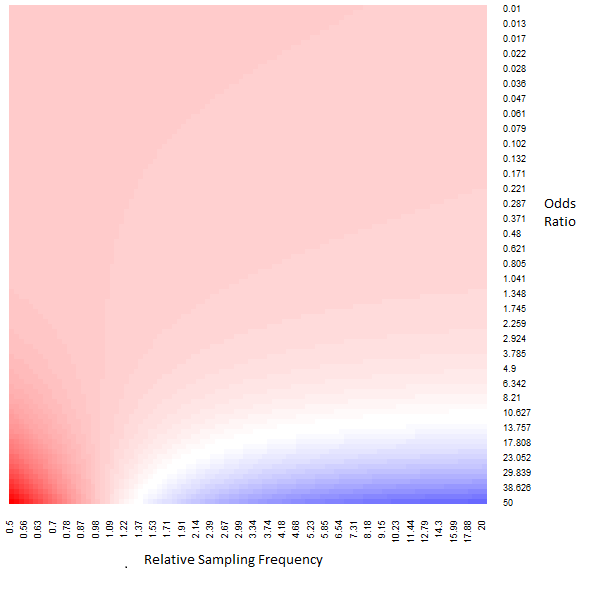
\includegraphics[width = 0.4\textwidth]{../methods/figs/mem_heatmap_article.png}
\caption{Measurement-error data quality adjustment: relative frequency $f_1/f_0$ (x-axis) against odds ratio (y-axis) for $FP=0.15$ and $FN=0.10$. Color scaled so blue = $-6$, white = 0, and red = $6$.}
\end{wrapfigure}




For fixed prevalence,


The first term is the same as before but increased by $(1 + FP + FN)$ to account for the additional uncertainty due to measurement-error.  The second term is the interaction between selection bias and measurement error.  Interestingly we can show that the sign is reversed, i.e., $sgn(\rho_{I,PZ}) = 1 - sgn(\rho_{I,Y})$, leading to an absolute \emph{reduction} in the error.

For this adjusted estimate, we can see that the directionality is maintained.  Therefore, the benefit is if the expected correlation is positive, we can feel like the estimate is likely an over-estimate and vice versa.  You pay a penalty in terms of variance and therefore the MSE may not be much smaller (CHECK!)

The effective sample size can then be bounded by
$$
n_{eff} = \frac{f}{1-f} \times E_{I} \left[ \rho_{I,Y}^2 D_M^2 \right]
$$

\subsection{Testing strategies and population size: a tango}

Data analysts have argued whether

Increasing testing under test rationing lowers correlation.  Example in Michigan and try and find CA and NY numbers.  Then show that this may cause higher FPs (cite antibody studies).

Plot Michigan tests per million and positives.  Next to NY.  Both as of April moved to prioritized sampling for symptomatic individuals.

\subsection{Cross-country comparisons}

So we can't estimate prevalence.  Can we not get a decent comparison?
$$
y_1 - y_2 = \frac{N_1}{n_1} ( \bar y_1 - Y_{1}) + \left( \frac{N_1}{n_1} Y_{1} - \frac{N_2}{n_2} Y_2  \right).
$$
OK then we should compare relative counts?
The question is then ``What are you comparing at a populatoin level?''
$$
y_1/N_1 - y_2/ N_2 = \left[ f_1 \sigma_{Y_1} \rho_{I_1, Y_1} \sqrt{\frac{1-f_1}{f_1}} D_{M_1} - f_2 \sigma_{Y_2} \rho_{I_1, Y_1} \sqrt{\frac{1-f_1}{f_1}}  \right] + \left[ f_1 \bar Y_1 - f_2 \bar Y_2 \right]
$$
Is this a quantity of genuine interest? Under SRS, this makes sense if $f_1 = f_2$.  Otherwise, you are comparing apples and oranges.  With selection bias, it's not clear that agreement in this quantity is even desirable.

$$
\frac{n}{N} \times \rho_{I,Y} \times \sqrt{\frac{1-f}{f}} \times \sigma_{Y} \times D_M
$$


\subsection{Ration-based testing allocation}

We assume that the percentage of tests is rationed according to severity of symptoms.

Note that a person who displays severe symptoms may be COVID negative.  This gives us a sense of the data quality.

\emph{Increasing testing leads to lower correlation in}

\subsection{Estimation of Data Quality}

We estimate $\rho$ using old and new methods.  Current SRS in US are weak.  So we just use my back of the envelope calculation. Tests per million as proxy since everyone is doing rationing. Cluster.

\subsection{Regrettable rates}

The data analyst, now wary of estimating prevalence and total counts, pauses and thinks.  They retur  n shortly thereafter, a bit agitated but still  \emph{Ok, perhaps total counts is a lost cause. Certainly, however, we can estimate the rate of growth.  All I want to know is when we hit the point at which the curve flattens and number of deaths decrease.  That can't be too hard, surely!}

The parameter $R_0$ in the ubiquitous SIR (susceptible-)

Ratio estimator $\bar y_2/ \bar y_1$.

Taylor series expansion:

$$
\begin{aligned}
\frac{\bar y_2}{\bar y_1} - \frac{\bar Y_2}{\bar Y_1}
&= \frac{\bar Y_2}{\bar Y_1} \left[ \rho_{I_2, Y_2} \sqrt{\frac{1-f_2}{f_2}} CV(Y_2)  - \rho_{I_1,Y_1} \sqrt{\frac{1-f_1}{f_1}} CV (Y_1) \left[ \rho_{I_2, Y_2} \sqrt{\frac{1-f_2}{f_2}} CV(Y_2) + 1 \right] \right]
\end{aligned}
$$

Supposing the sampling rate is constant, and

We talk about wanting to know if we are at the peak.  Let's define that time as when $\bar Y_2 / \bar Y_1 = 0$.  Then $\mu_{Y_1} = \mu_{Y_2} = \mu$ and $\sigma_{Y_1} = \sigma_{Y_2} = \sigma$. If selection at each time is independent and the selection process is stationary, we have bias of
$$
\rho \sqrt{\frac{1-f}{f}} \sigma \sqrt{\frac{1-\mu}{\mu}} \left[ \sqrt{\frac{1-\mu}{\mu}} - \rho \sqrt{\frac{1-f}{f}} \right ]
$$

If we collect $f = 0.01$ and the peak occurs at $\mu = 0.03$ with selection bias of $\rho = 0.05$. $1/\rho^2 \times (\mu/(1-\mu))^4$

Then we can be even further off than the prevalence by a factor of the odds ratio!

Suppose we collected $f=1/2$ and peak occurs at $\mu = 0.10$ and $\rho = 0.005$, then $9-\rho 3 = 9 - 0.005 \times 3 = 8.985$ and

{\bf How many days of dropping to guarantee it has decreased}

What is the effective sample size for these tests?

\subsubsection{Rate comparisons: a compounding mess}

\subsection{Testing increase changes data quality}

Many (cites) hve

\emph{Increasing testing leads to lower correlation only if we see the gap $\Delta$ decrease.  If we just see $f$ }

\subsection{Clinical trials}

Random sampling negates effect modifiers.  Random treatment assignment negates unobserved confounders.  Show simple example where $E[U]$ is high due to sampling bias and therefore you will think that the effect is significant! But it's because of sampling bias. Requires poststratification.

\subsection{Death counts}

\subsection{Stratified setting}


\section{Brief discussion of model-based approaches}

Here we explain a general state-space process model as compared to the measurement-process.  While related, the distinction drives our key results.

Observer controls testing, FP and FN.  Patients

Their behavior may depend on forecasts and therefore the notion of a counterfactual is not well defined.  For example, suppose an highly prominent model....

The transition from susceptible to infected is a complex function.  It is based on personal choices;  the second choice
$B$

\emph{Non-identifiable} and rely on assumptions.  As per Cox's statement.

This makes models \emph{fragile} and rely on strong data-generating assumptions.  In these settings data integration

\section{Stratified sampling: improving precision in low-prevalence environments}

Sampling network is hard.  Sampling high-risk strata is easy.  Simple example.
DTR and network connectivity is useful for understanding spread and where "testing should go".

\section{Decision-making: data versus information.}

Above we point to flaws in using observed data to reason about the

\section{That which does not break us, makes us stronger (but potentially not smarter)}

A slightly altered version of Nietzsche's famous quote has become a mantra for post-pandemic thinking: \emph{That which which does not break us, makes us stronger}.  While potentially true via viral resistance, it is not clear that governments have yet to learn lessons on pandemic response.

During the current wave, understanding prevalence is key.  It helps us determine long-term risk for a community and make targeted interventions.  This will allow
When prevalence is below a certain threshold, we can return to daily life.

Once we ``return to normal''\footnote{or at least the new normal}, it is clear that testing strategies should focus on early detection, heading off future outbreaks.
\emph{Anyone who wishes to go back to work}.  While laudable, without complete compliance, we may be riddles with selection bias and measurement-error.  This ignores even the practical and ethical quandaries of how to .

What do we do when we are faced with?  We design experiments with our objectives in mind.

(A) Prevalence: Targeted shutdowns
(B) Risk Detection: Contact tracing and altering

Use prior results to show that ratio estimator under SRS is a good predictor of potential outbreak.

``Disease free''


\section{Conclusion}

Interventions in this area are designed experiments.  Unlike Fischer's null, here the objectives are settings, statisticians.

Account for data quality in models by incorporating auxiliary information.  Perform advanced sensitivity analysis.  Forecasts should be called coutnerfactual forecasts.

\appendix

\section{Imperfect testing: derivation}

We considered the mean estimator
$$
\bar y_n^\star = \frac{\sum_{j=1}^N Y_j^\star I_j}{\sum_{j=1}^N I_j} = \frac{\sum_{i=1}^N  I_j Y_j^\star }{\sum_{j=1}^N  I_j } = \frac{\sum_{i=1}^N  I_j \left[ Y_j (1-P_j) + (1-Y_j) P_j \right]}{\sum_{j=1}^N  I_j }
$$
For any set of numbers $\{ A_1, \ldots, A_N \}$ we can view it as the support of a random variable $A_J$ induced by the random index $J$ defined on $\{1,\ldots, N\}$.  When $J$ is uniformly distributed $E_J (A_J) = \sum_{j=1}^N A_j / N \equiv \bar A_N$. Then
$$
\begin{aligned}
\bar y_n^\star  - \bar Y_N &= \frac{E_J \left[ I_J \left[ Y_J (1-P_J) + (1-Y_J) P_J \right] \right]}{E_J [ I_J ] } - E_J[Y_J] \\
&= \frac{E_J \left[ I_J P_J (1-2Y_J) \right]}{E_J [ I_J ] } + \left( \frac{E_J [I_J Y_J]}{E_J [ I_J ] } - \frac{E_J[Y_J] E_J[I_J]}{E_J[I_J]} \right) \\
\end{aligned}
$$
The term in parentheses can be re-written as
$$
\begin{aligned}
\frac{E_J [I_J Y_J]- E_J[Y_J] E_J[I_J]}{E_J[I_J]} &=  \frac{E_J [I_J Y_J]- E_J[Y_J] E_J[I_J]}{\sqrt{V_J(I_J) V_J(Y_J)}} \frac{\sqrt{V_J(I_J)}}{E_J[I_J]} \times \sqrt{V_J(Y_J)} \\
&= \rho_{I,Y} \times \sqrt{\frac{(1-f)}{f}} \times \sigma_Y
\end{aligned}
$$
which agrees with Meng's (2019) decomposition. For the other term, first we define $Z_j := 1 - 2 Y_j $. Then $Z_j = 1$ if $Y_j = 0$ and $Z_j = -1$ if $Y_j = 1$. Then the term can be re-written as
$$
\begin{aligned}
\frac{E_J \left[ I_J P_J (1-2Y_J) \right]}{E_J [ I_J ] } &= \left( \frac{E_J \left[ I_J P_J Z_J \right]}{E_J [ I_J ] } -  \frac{E_J \left[ P_J Z_J \right] E_J[ I_J]}{E_J [ I_J ] } \right) +  \frac{E_J \left[ P_J Z_J \right] E_J[ I_J]}{E_J [ I_J ] } \\
\end{aligned}
$$
The term in parentheses can be re-expressed using the previous technique as:
$$
\rho_{I, PZ} \times \sqrt{\frac{1-f}{f}} \times \sigma_{PZ}
$$
where now the ``data defect'' and ``problem difficulty'' are with respect to $PZ$ rather than $Y$. The final term is equal to
$$
\begin{aligned}
E_J [P_J Z_J ] &= E_J [ E_J [ P_J Z_J \mid Y_J ] ] \\
&= \pr (P = 1 \mid Y = 0) (1-\bar Y) - \pr(P=1 \mid Y = 1) \bar Y \\
&= FP - (FP + FN) \cdot \bar Y
\end{aligned}
$$
Combining these yields:
$$
\bar y_n^\star - \bar Y = \sqrt{\frac{1-f}{f}} \left[\rho_{I,Y} \sigma_Y + \rho_{I, PZ} \sigma_{PZ} + \sqrt{\frac{f}{1-f}} \left( FP - (FP+FN) \bar Y \right) \right]
$$
For the binary outcome $Y$, we have $\sigma_Y = \sqrt{\bar Y (1-\bar Y)}$. Moreover,
$$
\begin{aligned}
V_J(P_J Z_J) &= E_J[(P_J Z_J)^2] - E[P] E[Z] \\
&= E[P] - E[P] (1 - 2 \bar Y) = 2 \bar Y E_J [ P_J ] \\
&= 2 \bar Y \left( FP (1-\bar Y) + FN \bar Y \right) \\
\Rightarrow \sigma_{PZ} &= \sqrt{ 2 \bar Y \left( FP (1-\bar Y) + FN \cdot  \bar Y \right) }
\end{aligned}
$$
Then the formula for the error is given by:
$$
\sqrt{\frac{1-f}{f}} \left[\rho_{I,Y} \sqrt{\bar Y (1-\bar Y)} + \rho_{I, PZ} \sqrt{ 2 \bar Y \left( FP (1-\bar Y) + FN \cdot \bar Y \right )} + \sqrt{\frac{f}{1-f}} \left( FP - (FP+FN) \bar Y \right) \right]
$$

\subsection{Simple cases}

We consider two simple cases here.  First, we assume no false positive results, i.e., set $FP=0$.  Then $\sigma_{PZ} = \bar Y \sqrt{2 FN}$.  Then the math simplifies:
$$
\bar y_n^\star - \bar Y = \bar Y \sqrt{\frac{1-f}{f}} \left[\rho_{I,Y} \sqrt{\frac{1-\bar Y}{\bar Y}} + \sqrt{FN} \left( \sqrt{2} \rho_{I, PZ} - \sqrt{\frac{f}{1-f}} \sqrt{FN} \right)  \right]
$$
The sign of the error therefore depends on true data quality ($\rho_{I, Y}$), odds ratio, observed data quality~$\rho_{I,PZ}$, false negative rates (FN), and sample fraction $f$.

Second, we assume no false negative results, i.e., set $FN=0$.  Then $\sigma_{PZ} = \sqrt{2 FP \bar Y (1-\bar Y)}$.  Then the math simplifies:
$$
\bar y_n^\star - \bar Y = \sqrt{\bar Y (1-\bar Y)} \sqrt{\frac{1-f}{f}} \left[\rho_{I,Y} +  \sqrt{FP} \left( \sqrt{2} \rho_{I, PZ} + \sqrt{\frac{f}{1-f}} \sqrt{FP} \sqrt{1-\bar Y} \right)  \right]
$$
The sign of the error therefore depends on true data quality ($\rho_{I, Y}$),  observed data quality~$\rho_{I,PZ}$, false positive rates (FP), one minus prevalence ($1-\bar Y$), and sample fraction $f$.

\subsection{Adjusted estimator}

Define $\bar y_n^{\star \star} = \bar y_n^\star + FN \bar y_n^\star - FP(1-\bar y_n^\star)$; then the error is
$$
\bar y_n^{\star \star} - \bar Y = \sqrt{\frac{1-f}{f}} \left[ \rho_{I, Y} \sigma_{Y} (1+FP+FN)  + \rho_{I, PZ} \sqrt{ 2 \bar Y \left( FP (1-\bar Y) + FN \bar Y \right)} \right]
$$
In the case when false negative rate is zero, we have
$$
\bar y_n^{\star \star} - \bar Y = \sqrt{\frac{1-f}{f}} \sqrt{\bar Y(1-\bar Y)} \left[ \rho_{I, Y} (1+FP) + \rho_{I, PZ} \sqrt{ 2 FP } \right]
$$
In the case when false positive rate is zero, we have
$$
\bar y_n^{\star \star} - \bar Y = \sqrt{\frac{1-f}{f}} \sqrt{\bar Y(1-\bar Y)} \left[ \rho_{I, Y} (1+FN) + \rho_{I, PZ} \sqrt{ 2 FN } \times \sqrt{\frac{\bar Y}{1-\bar Y}} \right]
$$


\subsection{Estimate of observed data quality}

$$
\begin{aligned}
\rho_{I,PZ} &= \frac{C(I, PZ)}{\sqrt{V(PZ) V(I)}} \\
&= \frac{C(I, PZ)}{\sqrt{V(Y) V(I)}} \sqrt{\frac{V(Y)}{V(PZ)}} \\
&= \rho_{I,Y} \frac{C(I,PZ)}{C(I,Y)} \sqrt{ \frac{(1-\bar Y)}{2 ( FP (1-\bar Y) + FN \cdot \bar Y)} }
\end{aligned}
$$

$$
\begin{aligned}
C(I, PZ) &= E[ I P Z ] - E[I] E[PZ] \\
&=  [FP f_0 - (FP f_0 + FN f_1) \bar Y] - f [ FP - (FP+FN) \bar Y ] \\
&=  - FP \Delta \bar Y + FP \bar Y^2 \Delta - FN \bar Y^2 \Delta \\
&=  - \Delta \bar Y (FP \cdot (1-\bar Y) + FN \cdot \bar Y) \\
\end{aligned}
$$
where $f = f_1 \bar Y + f_0 (1-\bar Y)$ so $f_0 - f = -\Delta \bar Y$ and $f_1 - f = \Delta (1-\bar Y)$.
$$
\begin{aligned}
C(I, Y) &= E[ I Y ] - f \bar Y \\
&=  f_1 \bar Y + f_0 (1-\bar Y) - f \bar Y \\
&=  f_0 (1-\bar Y) + \Delta (1-\bar Y) \bar Y \\
&= (1-\bar Y) (f_0 + \Delta \bar Y)
\end{aligned}
$$
Combining yields
$$
\begin{aligned}
\rho_{I,PZ} &= \rho_{I,Y} \times \frac{- \Delta \bar Y (FP \cdot (1-\bar Y) + FN \cdot \bar Y) }{(1-\bar Y) (f_0 + \Delta \bar Y)} \times \sqrt{ \frac{(1-\bar Y)}{2 ( FP (1-\bar Y) + FN \cdot \bar Y)} } \\
&= - \rho_{I, Y} \times \Delta \times \sqrt{\frac{\bar Y}{1-\bar Y}} \frac{\sqrt{FP(1-\bar Y) + FN \cdot \bar Y}}{f_0 (1-\bar Y) + f_1 \bar Y} \times \sqrt{\frac{\bar Y}{2}}
\end{aligned}
$$
We can then re-write $\rho_{I,Y} \sigma_Y + \rho_{I,PZ} \sigma_{PZ}$ as
$$
\rho_{I,Y} \sigma_Y \left( 1 - \Delta \times \frac{\bar Y}{1-\bar Y} \times \frac{FP(1-\bar Y) + FN \cdot \bar Y}{f_0 (1-\bar Y) + f_1 \bar Y} \right)
$$
Suppose $f_1 = M \cdot f_0$.  Then $\Delta = f_1 - f_0 = f_0 (M-1)$ and $f_0 (1-\bar Y) + f_1 \bar Y = f_0 ( (1-\bar Y) + M \bar Y )$ and we can re-write above as
$$
\rho_{I,Y} \sigma_Y \left( 1 - (M-1) \times \frac{\bar Y}{1-\bar Y} \times \frac{FP(1-\bar Y) + FN \cdot \bar Y}{(1-\bar Y) + M \bar Y} \right).
$$

\subsection{Ratio estimator}

$$
\begin{aligned}
\frac{\bar y_2}{\bar y_1} - \frac{\bar Y_2}{\bar Y_1}
&= \frac{\bar y_2}{\bar Y_1  \left(1 + \rho_{I_1,Y_1} \sqrt{\frac{1-f_1}{f_1}} CV (Y_1) \right) } - \frac{\bar Y_2}{\bar Y_1}  \\
&\approx \frac{\bar y_2}{\bar Y_1} \left(1 - \rho_{I_1,Y_1} \sqrt{\frac{1-f_1}{f_1}} CV (Y_1) \right) - \frac{\bar Y_2}{\bar Y_1} \\
&= \frac{1}{\bar Y_1}  \rho_{I_2, Y_2} \sqrt{\frac{1-f_2}{f_2}} \sigma_{Y_2} - \frac{\bar y_2}{\bar Y_1} \cdot \rho_{I_1,Y_1} \sqrt{\frac{1-f_1}{f_1}} CV (Y_1).
\end{aligned}
$$
Focusing on the second term, we have
$$
\begin{aligned}
\frac{\bar y_2}{\bar Y_1} \cdot \rho_{I_1,Y_1} \sqrt{\frac{1-f_1}{f_1}} CV (Y_1) &= \frac{1}{\bar Y_1} \cdot \rho_{I_1,Y_1} \sqrt{\frac{1-f_1}{f_1}} CV (Y_1) \left[ \bar y_2 - \bar Y_2 + \bar Y_2 \right] \\
&= \frac{1}{\bar Y_1} \cdot \rho_{I_1,Y_1} \sqrt{\frac{1-f_1}{f_1}} CV (Y_1) \left[ \rho_{I_2, Y_2} \sqrt{\frac{1-f_2}{f_2}} \sigma_{Y_2} + \bar Y_2 \right] \\
&= \frac{\bar Y_2}{\bar Y_1} \cdot \rho_{I_1,Y_1} \sqrt{\frac{1-f_1}{f_1}} CV (Y_1) \left[ \rho_{I_2, Y_2} \sqrt{\frac{1-f_2}{f_2}} CV(Y_2) + 1 \right] \\
\end{aligned}
$$
Combining these we have
$$
\frac{\bar Y_2}{\bar Y_1} \left[ \rho_{I_2, Y_2} \sqrt{\frac{1-f_2}{f_2}} CV(Y_2)  - \rho_{I_1,Y_1} \sqrt{\frac{1-f_1}{f_1}} CV (Y_1) \left[ \rho_{I_2, Y_2} \sqrt{\frac{1-f_2}{f_2}} CV(Y_2) + 1 \right] \right]
$$
Under the assumption that the data quality and the sampling fraction are constant across time, this can be simplified
$$
\rho \times \sqrt{\frac{1-f}{f}} \times \frac{\bar Y_2}{\bar Y_1} \left[ \bar Y_1 - \bar Y_2 - (1-\bar Y_1)(1-\bar Y_2) \rho \sqrt{\frac{1-f}{f}} \right]
$$


\section{Quotes}

I prefer to think of a statistical sensibility rather than statistical thinking. It’s “less than an agenda but more than an attitude.”  It allows for methodological preference while avoiding dogma. Paired with data analytic humility and I think you have proper “data science”

“Routine statistical questions are less common than questionable statistical routines...” McCullagh (2005).

If an issue can be addressed nonparametrically then it will often be better to tackle it parametrically; however, if it cannot be resolved nonparametrically then it is usually dangerous to resolve it parametrically.” (p.96)

A test of meaningfulness of a possible model for a data-generating process is whether it can be used directly to simulate data.” (p.104).  In our current setting, this most certainly related to simulation while accounting for measruement error.




\end{document}